\section{Beispiele}
\subsection{Implementierung eines Zustandsautomaten}
Zwei Beispiele zeigen die Verwendung von Intervall-Events bei der
Implementierung von Zustandsautomaten. Zustandsautomaten k"onnen hervoragend
durch die Verwendung von IntervallEvents implementiert werden, da
Zustandsautomaten immer vom Zustand abh"anige Reaktionen auf Events zeigen.

Zur Implementierung kann jeder Zustand des Automaten als ein Intervall
abgebildet werden. Nun kann man Entry-Actions als before-Event an ein Intervall
und Exit-Actions als ein after-Event an das Intervall binden. Transition-Actions
k"onnen wahlweise an das Before- oder das After-Event gebunden werden.
Self-Transitions werden als Vereinigung zwischen dem Intervall-Event und dem
ausl"osenden Event der Self-Transition abgebildet. 

Durch diese Vorgehensweise ergibt sich eine bessere Wartbarkeit des
Quellcodes, da das Programmverhalten nicht mehr imperativ durch If-Statements
oder das Statemachine-Pattern beschrieben wird. Viel mehr wird das
Programmverhalten deklarativ durch Intevall-Events spezifiziert.

Im Rahme dieser Arbeit wurden zwei Zustandsautomaten implementiert. Bei dem
ersten Zustandsautomaten handelt es sich um das vereinfachte Verhalten eines
Filetransfer-Servers dessen Verbindungen offen oder geschlossen sein k"onnen. Der
resultierende Zustandsautomat ist in Abb\ref{filetransfer_behaviour} zu sehen.

%\usepackage{graphics} is needed for \includegraphics
\begin{figure}[htp]
\begin{center}
  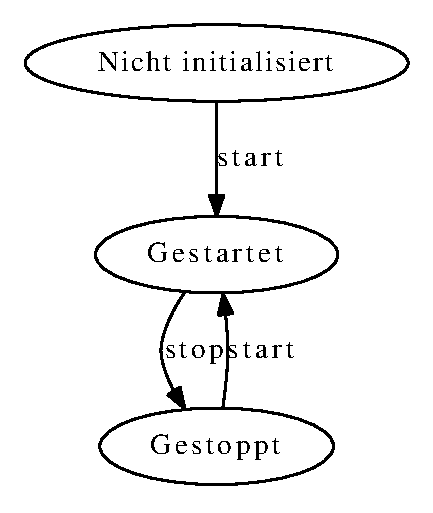
\includegraphics[width=0.15\textwidth]{graphics/tcp_stm.dot.eps}
  \caption{Verhalten einer Filetransfer-Verbindung}
  \label{filetransfer_behaviour}
\end{center}
\end{figure}

\subsubsection{SimpleWebshop-Verhalten}

%\usepackage{graphics} is needed for \includegraphics
\begin{figure}[htp]
\begin{center}
  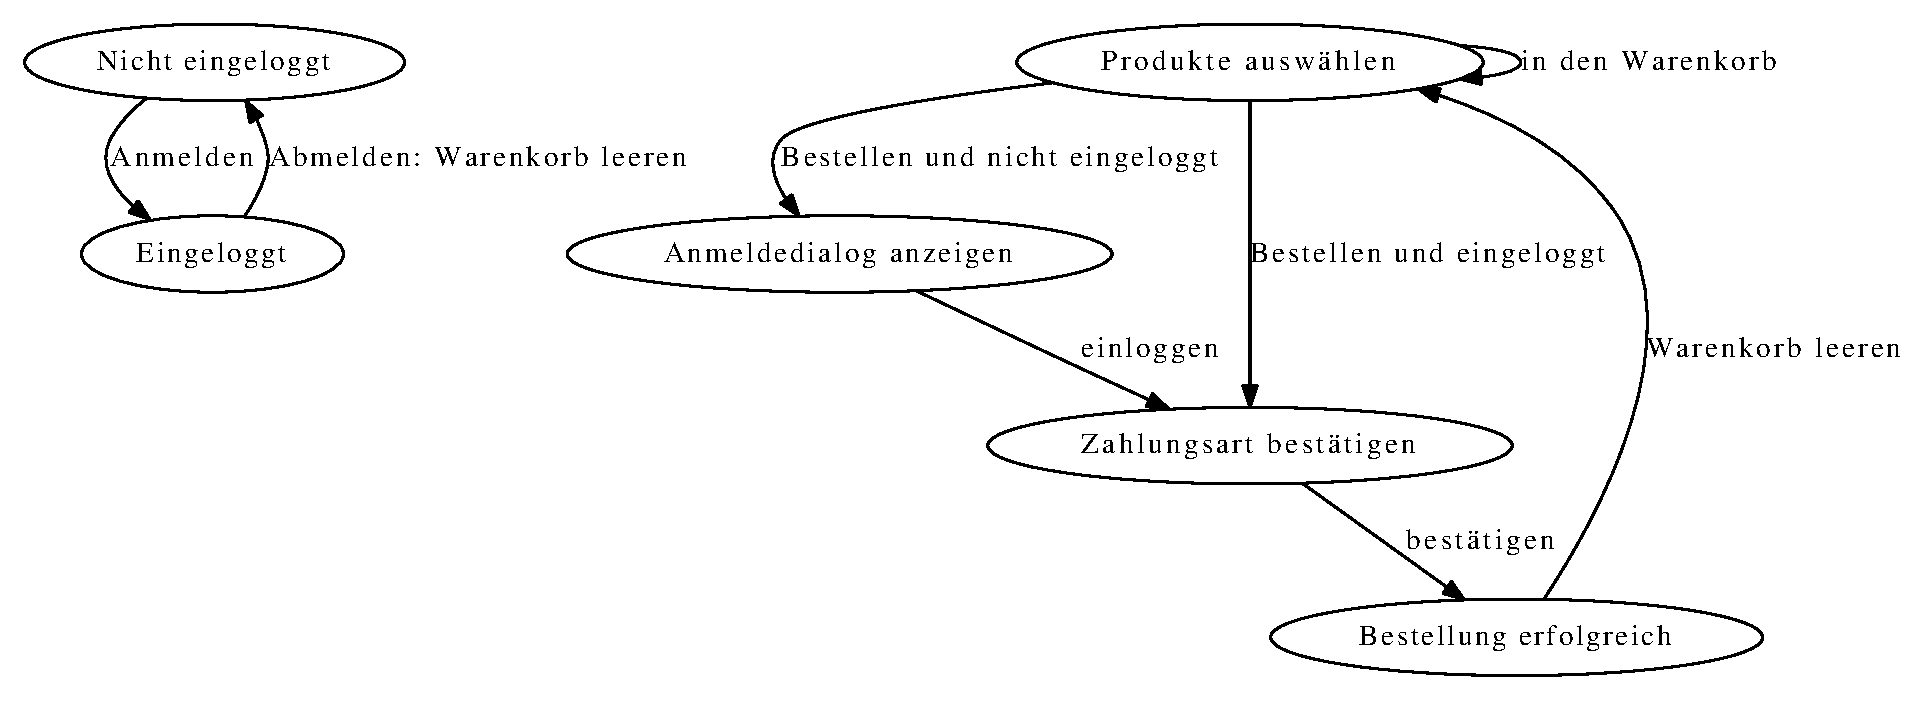
\includegraphics[width=0.6\textwidth]{graphics/webshop.dot.eps}
  \caption{Bestellvorgang in einem Web-Shop}
  \label{webshop_behaviour}
\end{center}
\end{figure}